
%%%%%%%%%%%%%%%%%%%%%%%%%%%%%%%%%%%%%%%%%%%%%%%%%%%%%%%%%%{
%\documentclass[twoside,11pt]{article}
\documentclass[UTF8]{ctexart}
%%%%% PACKAGES %%%%%%
\usepackage{pgm2016}
\usepackage{amsmath}
\usepackage{algorithm}
\usepackage[noend]{algpseudocode}
\usepackage{subcaption}
\usepackage[english]{babel}	
\usepackage{paralist}	
\usepackage[lowtilde]{url}
\usepackage{fixltx2e}
\usepackage{listings}
\usepackage{color}
\usepackage{hyperref}
\usepackage{mdframed}
\usepackage{xcolor,graphicx,float}

%\usepackage{auto-pst-pdf}
\usepackage{pst-all}
\usepackage{pstricks-add}

%%%%% MACROS %%%%%%
\algrenewcommand\Return{\State \algorithmicreturn{} }
\algnewcommand{\LineComment}[1]{\State \(\triangleright\) #1}
\renewcommand{\thesubfigure}{\roman{subfigure}}
\definecolor{codegreen}{rgb}{0,0.6,0}
\definecolor{codegray}{rgb}{0.5,0.5,0.5}
\definecolor{codepurple}{rgb}{0.58,0,0.82}
\definecolor{backcolour}{rgb}{0.95,0.95,0.92}
\lstdefinestyle{mystyle}{
	backgroundcolor=\color{backcolour},  
	commentstyle=\color{codegreen},
	keywordstyle=\color{magenta},
	numberstyle=\tiny\color{codegray},
	stringstyle=\color{codepurple},
	basicstyle=\footnotesize,
	breakatwhitespace=false,        
	breaklines=true,                
	captionpos=b,                    
	keepspaces=true,                
	numbers=left,                    
	numbersep=5pt,                  
	showspaces=false,                
	showstringspaces=false,
	showtabs=false,                  
	tabsize=2
}
\lstset{style=mystyle}

\newenvironment{problem}[2][问题]
{\begin{mdframed}[backgroundcolor=gray!20] \textbf{#1 #2} \\}
	{\end{mdframed}}

\newenvironment{dingyi}[2][定义]
{\begin{mdframed}[backgroundcolor=gray!20] \textbf{#1 #2} \\}
	{\end{mdframed}}

\newenvironment{dingli}[2][定理]
{\begin{mdframed}[backgroundcolor=gray!20] \textbf{#1 #2} \\}
	{\end{mdframed}}

%%%%%%%%%%%%%%%%%%%%%%%%%%%%%%%%%%%%%%%%%%%%%%%%%%%%%%%%%% 


%%%%%%%%%%%%%%%%%%%%Information%%%%%%%%%%%%%%%%%%%%%%%%%%%
\newcommand\course{sd03431280}
\newcommand\courseName{数值计算方法}
\newcommand\semester{2020·春季}
\newcommand\assignmentNumber{5}
\newcommand\studentName{陈路}
\newcommand\studentEmail{chenlu.scien@gmail.com}
\newcommand\studentNumber{201800301206}
\newcommand\addr{泰山学堂2018级计算机取向}
%%%%%%%%%%%%%%%%%%%%%%%%%%%%%%%%%%%%%%%%%%%%%%%%%%%%%%%%%%



%%%%%%%%%%%%%%%%%%%%%%%%%%%%%%%%%%%%%%%%%%%%%%%%%%%%%%%%%%
    \ShortHeadings{山东大学\quad \semester\quad  \course\quad \courseName}{\addr \quad \studentName \quad \studentNumber}
    \firstpageno{1}
    
    \begin{document}
    
    \title{第\assignmentNumber 章\quad 常微分方程数值解}
    
    \author{\name \studentName \email \studentEmail \\
    \studentNumber
    }
    
    \maketitle
%%%%%%%%%%%%%%%%%%%%%%%%%%%%%%%%%%%%%%%%%%%%%%%%%%%%%%%%%%

\section{上机实验题}

\begin{problem}{1}
	求
	\begin{align}
		y'=1 + y^2,\quad y(0)=0 \label{eq:p1}
	\end{align}
	的数值解(分别用欧拉显格式、梯形预估修正格式、4阶龙格库塔格式,并与解析解比较这三种格式的收敛性).
\end{problem}
\textbf{解}:\\
方程\ref{eq:p1}的精确解为$y(t)=tan(t)$,是一个周期为$\pi$的奇函数,我们不妨考察近似是其一个完整的最小周期的区间$[0,3]$.
欧拉格式的代码实现
\begin{lstlisting}[language=matlab]
	function E = euler(f, a, b, ya, M)
	% Input  - f    is the function entered as a string 'f'
	%        - a,b  are the left and right end points
	%        - ya   is the initial condition y(a)
	%        - M    is the number of steps
	% Output - E=[T' Y'] where T is the vector of abscissas and
	%               Y is the vector of ordinates
	
	h = (b-a)/M;
	T = zeros(1, M+1);
	Y = zeros(1, M+1);
	T = a:h:b;
	Y(1) = ya;
	for j = 1:M
		Y(j+1) = Y(j) + h * feval(f,T(j),Y(j));
	end
	E=[T' Y'];
	plot(T ,Y ,'r');
	end
\end{lstlisting}
实验结果如下表\ref{table:euler}\\
\begin{table}[h]
	\centering
	\caption{常微分方程\ref{eq:p1}在欧拉格式下步长$h=1, 0.5, 0.25$的输出结果}
	\label{table:euler}
	\begin{tabular}{lllll}
		\hline
		\multicolumn{1}{c}{\textbf{步长h}} & \multicolumn{1}{c}{\textbf{迭代次数M}} & \multicolumn{1}{c}{\textbf{y(1)的逼近}} & \multicolumn{1}{c}{\textbf{y(2)的逼近}} & \multicolumn{1}{c}{\textbf{y(3)的逼近}} \\ \hline
		1                                & 3                                  & 1                                    & 3                                    & 13                                   \\ \hline
		0.5                              & 6                                  & 1.1250                               & 5.306671142578125                    & 2.181344382569777e+02                \\ \hline
		0.25                             & 12                                 & 1.255186677910388                    & 13.793965310277061                   & 1.644599578587173e+10                \\ \hline
	\end{tabular}
\end{table}
将上表作图如下,其中红色曲线为方程\ref{eq:p1}使用欧拉格式在步长$h=1$时的计算结果,蓝色曲线为步长$h=0.5$时的计算结果,绿色曲线为步长$h=0.25$时的计算结果.
\begin{figure}[H]
	\centering
	\begin{minipage}[c]{0.5\textwidth}
		\centering
		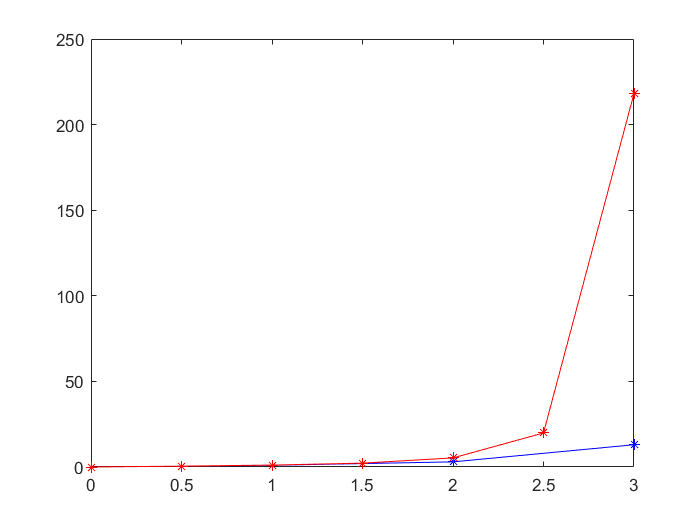
\includegraphics[width=0.7\columnwidth]{figures/p1euler1.png}
	\end{minipage}%
	\begin{minipage}[c]{0.5\textwidth}
		\centering
		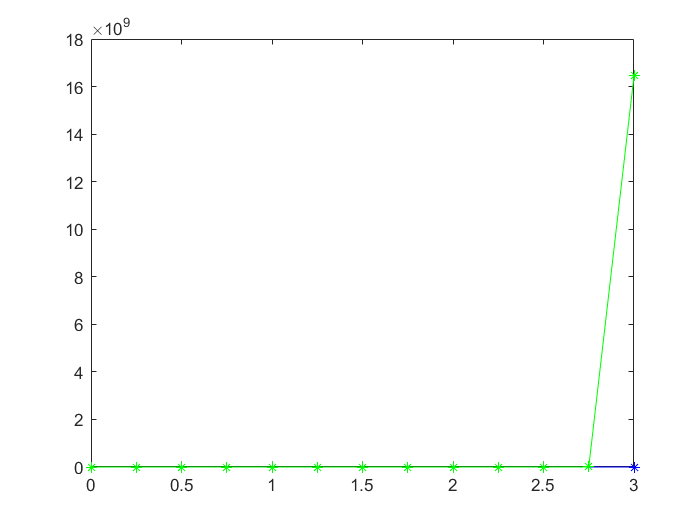
\includegraphics[width=0.7\columnwidth]{figures/p1euler2.png}
	\end{minipage}
	\caption{常微分方程\ref{eq:p1}在欧拉格式下步长$h=1, 0.5, 0.25$的输出结果比较}
\end{figure}
梯形格式的代码实现
\begin{lstlisting}[language=matlab]
	function H = heun(f, a, b, ya, M)
	% Input - f    is the function entered as a string 'f'
	%       - a,b  are the left and right end points
	%       - ya   is the initial condition y(a)
	%       - M    is the number of steps
	% Output - H=[T' Y'] where T is the vector of abscissas and
	%               Y is the vector of ordinates
	
	h = (b-a)/M;
	T = zeros(1, M+1);
	Y = zeros(1,M+1);
	T = a:h:b;
	Y(1) = ya;
	for j = 1:M
		k1 = feval(f, T(j), Y(j));
		k2 = feval(f, T(j+1), Y(j) + h*k1);
		Y(j+1) = Y(j) + (h/2)*(k1+k2);
	end
	H=[T' Y'];
	plot(T ,Y ,'r');
	end
\end{lstlisting}
实验结果如下表\ref{table:heun}\\
\begin{table}[h]
	\centering
	\caption{常微分方程\ref{eq:p1}在梯形格式下步长$h=1, 0.5, 0.25$的输出结果}
	\label{table:heun}
	\begin{tabular}{lllll}
		\hline
		\multicolumn{1}{c}{\textbf{步长h}} & \multicolumn{1}{c}{\textbf{迭代次数M}} & \multicolumn{1}{c}{\textbf{y(1)的逼近}} & \multicolumn{1}{c}{\textbf{y(2)的逼近}} & \multicolumn{1}{c}{\textbf{y(3)的逼近}} \\ \hline
		1                                & 3                                  & 1.500000000000000                    & 14.906250000000000                   & 2.847341394853592e+04                \\ \hline
		0.5                              & 6                                  & 1.514130592346191                    & 97.698983198999300                   & 7.746950417290489e+25                \\ \hline
		0.25                             & 12                                 & 1.539404774465156                    & 1.533032751706393e+05                & Inf                                  \\ \hline
	\end{tabular}
\end{table}
将上表作图如下,其中红色曲线为方程\ref{eq:p1}使用梯形格式在步长$h=1$时的计算结果,蓝色曲线为步长$h=0.5$时的计算结果,绿色曲线为步长$h=0.25$时的计算结果.
\begin{figure}[H]
	\centering
	\begin{minipage}[c]{0.5\textwidth}
		\centering
		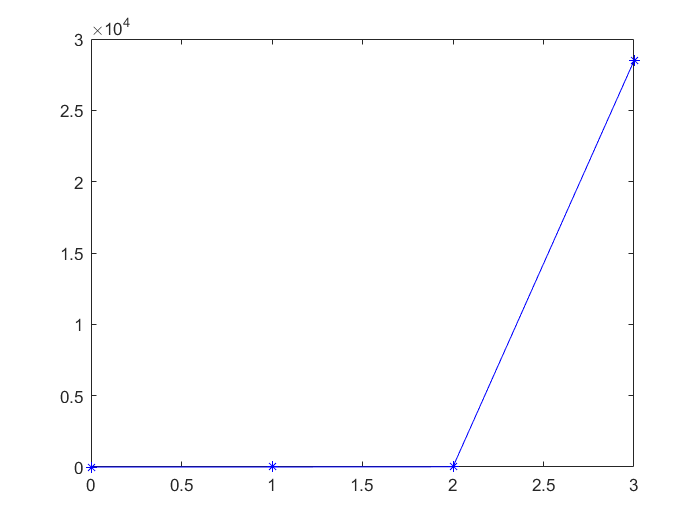
\includegraphics[width=0.7\columnwidth]{figures/p1heun1.png}
	\end{minipage}%
	\begin{minipage}[c]{0.5\textwidth}
		\centering
		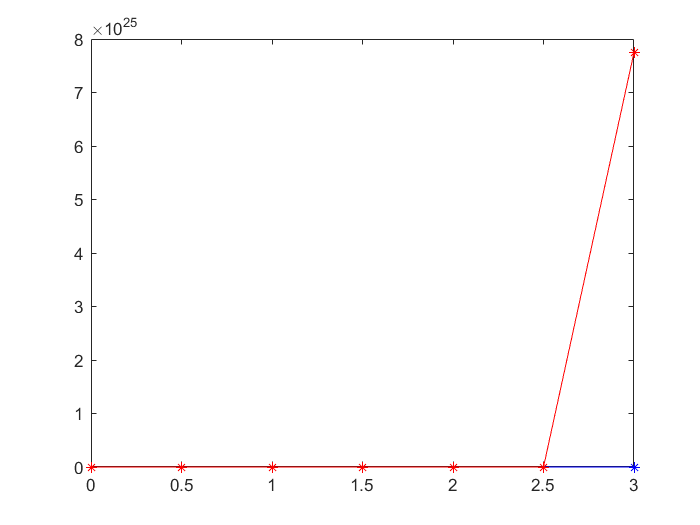
\includegraphics[width=0.7\columnwidth]{figures/p1heun2.png}
	\end{minipage}
	\begin{minipage}[c]{0.5\textwidth}
		\centering
		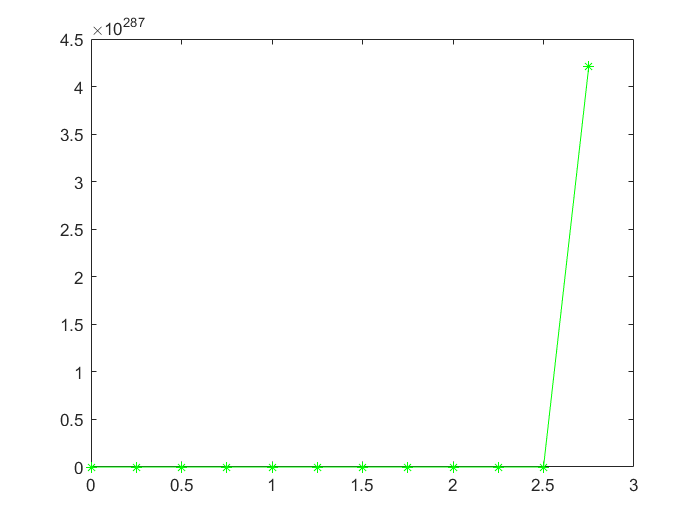
\includegraphics[width=0.7\columnwidth]{figures/p1heun3.png}
	\end{minipage}
	\caption{常微分方程\ref{eq:p1}在梯形格式下步长$h=1, 0.5, 0.25$的输出结果比较}
\end{figure}
4阶龙格库塔格式的代码实现
\begin{lstlisting}[language=matlab]
	function R = rk4(f, a, b, ya, M)
	% Input - f   is the function entered as a string 'f'
	%       - a,b are the left and right end points
	%       - ya  is the initial condition y(a)
	%       - M   is the number of steps
	% Output - R=[T' Y'] where T is the vector of abscissas
	%               Y is the vector of ordinates
	
	h = (b-a)/M;
	T = zeros(1, M+1);
	Y = zeros(1, M+1) ;
	T = a:h:b;
	Y(1) = ya;
	for j = 1:M
		k1 = h*feval(f, T(j), Y(j));
		k2 = h*feval(f, T(j)+h/2, Y(j)+k1/2);
		k3 = h*feval(f, T(j)+h/2, Y(j)+k2/2);
		k4 = h*feval(f, T(j)+h, Y(j)+k3);
		Y(j+1) = Y(j) + (k1 + 2*k2 + 2*k3 + k4)/6;
	end
	R=[T' Y'];
	plot(T ,Y ,'r');
	end
\end{lstlisting}
实验结果如下表\ref{table:rk}\\
\begin{table}[h]
	\centering
	\caption{常微分方程\ref{eq:p1}在4阶龙格库塔格式下步长$h=1, 0.5, 0.25$的输出结果}
	\label{table:rk}
	\begin{tabular}{lllll}
		\hline
		\multicolumn{1}{c}{\textbf{步长h}} & \multicolumn{1}{c}{\textbf{迭代次数M}} & \multicolumn{1}{c}{\textbf{y(1)的逼近}} & \multicolumn{1}{c}{\textbf{y(2)的逼近}} & \multicolumn{1}{c}{\textbf{y(3)的逼近}} \\ \hline
		1                                & 3                                  & 1.535847981770833                    & 5.177220263983291e+02                & 1.118005492535454e+39                \\ \hline
		0.5                              & 6                                  & 1.554612104179646                    & 1.112097692431962e+08                & Inf                                  \\ \hline
		0.25                             & 12                                 & 1.557247964295967                    & 6.627407669161920e+80                & Inf                                  \\ \hline
	\end{tabular}
\end{table}
将上表作图如下,其中红色曲线为方程\ref{eq:p1}使用4阶龙格库塔格式在步长$h=1$时的计算结果,蓝色曲线为步长$h=0.5$时的计算结果.
\begin{figure}[H]
	\centering
	\begin{minipage}[c]{0.5\textwidth}
		\centering
		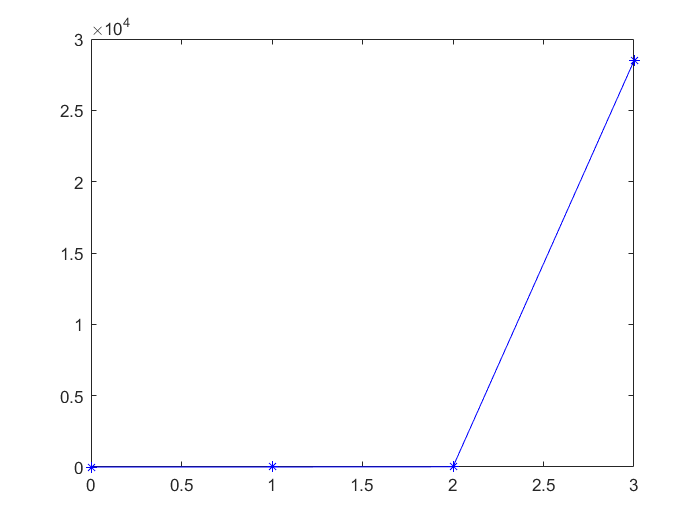
\includegraphics[width=0.7\columnwidth]{figures/p1heun1.png}
	\end{minipage}%
	\begin{minipage}[c]{0.5\textwidth}
		\centering
		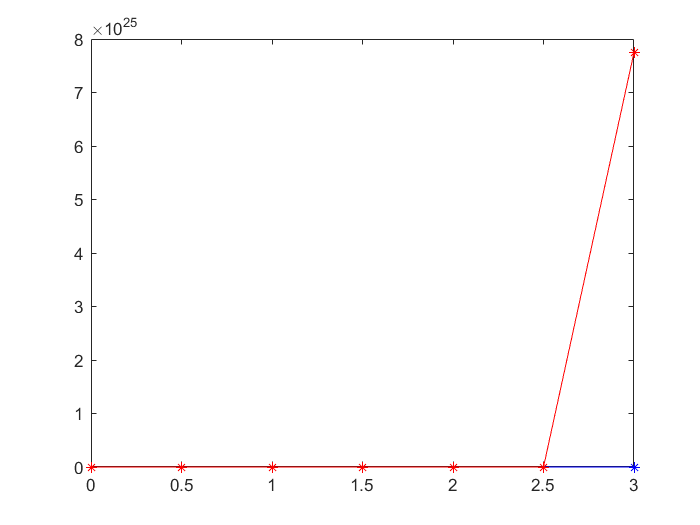
\includegraphics[width=0.7\columnwidth]{figures/p1heun2.png}
	\end{minipage}
	\caption{常微分方程\ref{eq:p1}在4阶龙格库塔格式下步长$h=1, 0.5$的输出结果比较}
\end{figure}


\begin{problem}{2}
	用龙格库塔4阶方法求解描述振荡器的经典的$van\quad der\quad Pol$微分方程
	\begin{align}
		\left\{\begin{array}{l}
		\frac{\mathrm{d}^{2} y}{\mathrm{d} t^{2}}-\mu\left(1-y^{2}\right) \frac{\mathrm{d} y}{\mathrm{d} t}+y=0 \\
		y(0)=1, y^{\prime}(0)=0
		\end{array}\right.\notag
	\end{align}
	分别取$μ = 0.01, 0.1, 1$,作图比较计算结果.
\end{problem}
\textbf{解}:\\
首先把二阶常微分方程化为常微分方程组. 设$y_1=y, y_2=y'$,则有:
\begin{align}
	\left\{\begin{array}{l}
		y_{1}'=y_2 \\
		y_{2}'=\mu (1-y^{2}_{1}y_{2}-y_{1}) \\
		y(0)=1, y^{\prime}(0)=0
	\end{array}\right.\label{eq:vdp}
\end{align}
描述该微分方程组的函数如下:
\begin{lstlisting}[language=matlab]
	function dy = vdp(t,y)
		dy = zeros(2,1);
		dy(1) = y(2);
		dy(2) = 0.01 * (1-y(1)^2)*y(2) - y(1); % change mu
	end
\end{lstlisting}
分别取$\mu = 0.01, 0.1, 1$,输出图形如下图\ref{fig:p2},其中蓝色曲线为$\mu = 0.01$时微分方程\ref{eq:vdp}的数值解,红色曲线为$\mu = 0.1$时的数值解,绿色曲线为$\mu = 1$时的数值解.\\
\begin{figure}[H]
	\begin{center}
		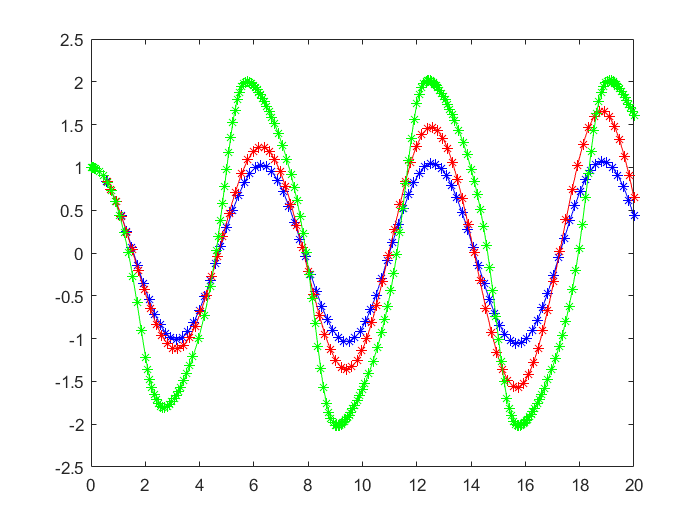
\includegraphics[width=0.7\columnwidth]{figures/p2.png}
		\caption{微分方程\ref{eq:vdp}在$\mu = 0.01, 0.1, 1$时的数值解}
		\label{fig:p2}
	\end{center}
\end{figure}
方程组在区间$[a,b]$上的四阶龙格库塔算法代码实现如下:
\begin{lstlisting}[language=matlab]
function [T, Z] = rks4(F, a, b, Za, M)
% Input - F    is the system input as a string 'F'
%       - a,b  are the end points of the interval
%       - Za   =[x(a) y(a)] are the initial conditions
%       - M    is the number of steps
% Output - T   is the vector of steps
%        - Z   =[x1(t). . .xn(t)]; where xk(t) is the approximation
%                   to the kth dependent variable

h = (b-a)/M;
T = zeros(1, M+1) ;
Z = zeros(M+1, length(Za));
T = a;h:b;
Z(1,:) = Za;
for j = 1:M
k1 = h * feval(F,T(j), Z(j,:));
k2 = h * feval(F, T(j)+h/2, Z(j,:)+k1/2);
k3 = h * feval(F, T(j)+h/2, Z(j,:)+k2/2);
k4 = h * feval(F, T(j)+h, Z(j,:)+k3);
Z(j+1,:) = Z(j,:) + (k1+2*k2+2*k3+k4)/6;
end
\end{lstlisting}

\end{document}
